\documentclass[runningheads]{llncs}
\usepackage[margin=1in]{geometry}

% Packages typically used
\usepackage{graphicx} % For images
\graphicspath{{images/}}
\usepackage[colorlinks=true, linkcolor=black, citecolor=blue, urlcolor=blue]{hyperref}
\usepackage{cite} % Better citation handling
\usepackage{amsmath}
\usepackage{amssymb}

\usepackage{algorithm}
\usepackage{algpseudocode}
\usepackage{float}

\usepackage{lipsum}
\usepackage{wrapfig}
\usepackage{subcaption}

\newcounter{rulecounter}
\setcounter{rulecounter}{1}
\newcommand{\psrule}[2]{%
	&\text{#1} &\rightarrow \text{#2} &\quad (\arabic{rulecounter})\\%
  \stepcounter{rulecounter}%
}

\begin{document}
%\flushbottom

\title{Love Languages: Reimagining English Syntax Trees as a Turing Complete Language}
\titlerunning{Love Languages}

\author{
	Cassidy Diamond
}

\authorrunning{C. Diamond}

\institute{
  Carnegie Mellon University \\
  \email{cass-diamond@protonmail.com}
}

\maketitle

\begin{abstract}
	This project reimagines the syntax structure of the English language as a Turing Complete programming language. I present a system to convert syntax trees into Brainfuck (bf) programs. Under this system, I then explore two approaches for converting bf programs into functionally-equivalent syntax trees. A final algorithm assigns words to completed programs and connects the results and processes of this project to Christopher Strachey's Love Letter Algorithm, thus positioning the work as a response to one of the first examples of computer-generated literature and as an instance of queer computer art.
\end{abstract}

The code for this project -- including exciting executables (!) -- can be found on \href{https://example.com}{my website}. %TODO
\section{Introduction}
In the Fall of 2022 I was an undergraduate sophomore, not yet formally a computer science student, and among other more interesting life developments during that period (like coming out, dating for the first time -- somehow relevant to this paper% TODO: do I want this?
), I was taking the linguistics course "Nature of Language" taught by Christina Bjorndahl. It was a typical introductory course on which I gladly used the last bit of my elective credits, a scarce resource otherwise sparingly spent. The majority of my future classes would be devoted to the technical requirements of either math or computer science. But linguistics was something I took interest to since high school and easily landed in my schedule. It was somewhere there in the milieu of morphemes, syntax, and phonetics, I had come across one of the topics central to this project and paper.
%TODO: image of a program/lover letter taped on the wall of Gates machine learning/langauge department
\subsection{X-Bar Theory}
Nature of Language introduced us to Phrase Structure Rules (PSRs), a series of rules that models the syntax of language. Our class used them as a way to differentiate sentence ambiguity. % For example, "We saw the woman with the telescope" takes on different meaning when the prepositional phrase "with the telescope" modifies the verb ("saw", in which case the telescope was a instrument the subject uses to see) versus the object determiner phrase ("the woman", in which case the woman is carrying a telescope).
For example, consider the phrase, "We saw the woman with the telescope". Are we seeing a woman through a telescope, or a woman who is carrying a telescope?

%\begin{wrapfigure}{r}{0.5\textwidth}
\begin{figure}
    \[
			\begin{array}{rlrr}
				S  &\rightarrow \text{DP} \quad \text{VP}&\textit{The quick brown fox jumps over the lazy dog} &\ \ (1) \\
			DP  &\rightarrow \text{D} \quad \text{N}_1&\textit{(the)$_\text{D}$ (quick brown fox)$_{\text{N}_1}$} & (2) \\
				\text{N}_1 &\rightarrow (\text{AP}+) \quad \text{N}_1 \quad (\text{PP}+)&\textit{(quick)$_\text{AP}$ (brown)$_\text{AP}$ fox} & (3)\\
				\text{VP} &\rightarrow \text{V}_1 \quad (\text{DP}) \quad (\text{PP})&\textit{(jumps)$_{\text{V}_1}$ (over the lazy dog)}_{\text{PP}} & (4)\\
				\text{PP} &\rightarrow \text{P} \quad \text{DP}&\textit{over the lazy dog} & (5)\\
    \end{array}
	\]
    \caption{Abbreviated Example of Phrase Structure Rules}
		\label{fig:psr}
\end{figure}
%	\end{wrapfigure}
PSRs were first proposed by Noam Chomsky in 1957, then later expanded into X-bar theory, also a creation by Chomsky, in 1970. %TODO: citation
The rules in Figure \ref{fig:psr} show an abbreviated example what these a complete PSR system may look like. We interpret these as follows: By (1), we know a sentence is composed of a determiner phrase and a verb phrase. By (2), we know a determiner phrase is a determiner and a noun. By (3), a noun is optionally preceded by any quantity of adjective phrases (i.e both "quick" and "brown"), and optionally followed by any quantity of prepositional phrases.

From our earlier example, the syntax tree would therefore encode the difference between the prepositional phrase "with the telescope" modifying the noun phrase as in rule (3): "$(\text{woman})_{\text{N}_1}\ \text{(with the telescope)}_{\text{PP}}$" -- or the verb phrase as in rule (4): "saw $\text{(the woman)}_{\text{DP}}$ $(\text{with the telescope})_{\text{PP}}$".
% TODO: figure with two trees showing the two rules

X-Bar theory comes and simplifies these rules. While the exact motivations of these changes can be found elsewhere, %TODO: cittaion
a rule in X-bar theory is binary (meaning each node has exactly two children to it), and broken up into multiple levels to introduce a hierarchy. So for example, we may have a Noun Phrase at the phrasal level, an N' (pronounced N-bar) at the intermediate level, and an N at the word/head level.

\begin{figure}
	\centering
	\begin{subfigure}[b]{0.45\textwidth}
    \[
		\begin{array}{rllr}
			\text{Phrase level}\quad  &\text{NP}  &\rightarrow \text{N'}&\quad (1)\\
			\text{Intermediate level}\quad&\text{N'}  &\rightarrow \text{N'}&(2)\\
																		&\text{N'}  &\rightarrow \text{AP} \quad \text{N'}&(3)\\
																		&\text{N'}  &\rightarrow \text{N'} \quad \text{PP}&(4)\\
			\text{Head level}\quad&\text{N'}  &\rightarrow \text{N}&(5)\\
    \end{array}
	\]
    \caption{Abbreviated Example of X-Bar Rules}
		\label{fig:xbar}
	\end{subfigure}
	\begin{subfigure}[b]{0.45\textwidth}
		\centering
		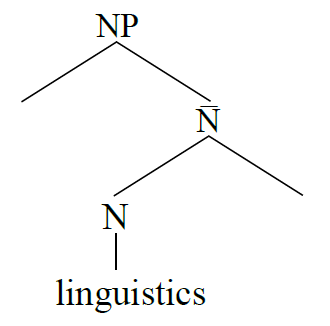
\includegraphics[height=10em]{nouns}
		\caption{Drawing rules (1), (2) and (5) in tree hierarchy}
		\label{fig:nouns-img}
	\end{subfigure}
	\caption{}
\end{figure}
When only one rule is given we still draw two children below each node as in Figure \ref{fig:nouns-img} .

We observe two key properties in PSR and X-Bar theory: First, there is a well-defined structure in the possible syntax trees that we can produce, given by the rules we start with. Second, the rules are capable of recursion -- that is, a rule can reference itself (for example, see rule (2) or (3) in Figure \ref{fig:xbar}). This structure suggests the inklings of a programming language, which also produces highly regulated and recursive forms.
\subsection{Well known homosexual: Alan Turing}
In a foundational paper to the study of computer science as a whole, in 1936 Alan Turing introduced the concept of the \textbf{Turing Machine} (TM), a physical model for computation. % TODO: citation
The Turing Machine receives as input an infinite tape of symbols. At any moment the machine reads a single symbol -- referred to as the scanned symbol -- and based on \textit{only} that symbol can then perform several pre-determined options: moving the tape to the left by some number of symbols, to the right, or writing a new symbol in place.

The \textbf{Church-Turing thesis} % TODO: citation
expands upon this, and essentially posits that a Turing Machine is capable of solving any problem that can be computed by an algorithm; and that if there is an algorithm that can solve a problem, then it can be ran by a Turing Machine.\footnote{The concept of a "computable" problem is actually formally defined by what a TM can solve making my use of it somewhat circular, but intuitively, it's any problem a human can solve by following instructions and aided by pen \& paper.}

A programming language or rule set is called \textbf{Turing Complete} if it can simulate a Turing Machine, and by the Church-Turing thesis, we know that such languages can determine the solution to any problem that is computable at all -- that is, in terms of which problems they can solve, all Turing-Complete languages are strictly equivalent.

The connection between PSR and X-Bar rules to Turing Machines is not a stretch; certain Cellular Automata (CA), such as Conway's Game of Life, are also known to be Turing Complete and exhibit similar properties. %TODO: citation
In CA, an initial set of rules determines exactly how each state progresses, likened to the syntax rules given by X-Bar theory. Furthermore, recursive properties also arise CA in that some cell structures of can replicate themselves or "loop" in their configuration, again similar to the often recursive nature of syntax rules in language.

\subsubsection{Brainfuck}
Besides a TM or CA, another popular Turing Complete instruction set is brainfuck (bf). Instead of an infinite tape, the language utilizes an array of (in its original specification) 30,000 byte cells initialized to zero, an input channel to receive initial bytes, an output channel to write bytes to, and a data-pointer which indicates which position in the array is "active".

The bf language uses eight operations to affect these data structures, given by Table \ref{table:bf} . An input program is a series of these operations/instructions, each being executed sequentially unless otherwise noted.
\begin{table}[H]
\begin{tabular}{l|l}
\textbf{Operation} & \textbf{Action Performed}                                                                \\ \hline
\textgreater{}     & Move the data pointer to the right                                                       \\
\textless{}        & Move the data pointer to the left                                                        \\
+                  & Increment the data pointer                                                               \\
-                  & Decrement the data pointer                                                               \\
{[}                & If the active byte is zero, jump to the operation \textit{after} the next {]} character           \\
{]}                & If the active byte is not zero, move to the operation \textit{before} the preceding {[} character \\
.                  & Output the active byte to the output channel                                             \\
,                  & Set the active byte to be equal to the next byte in the input channel
\end{tabular}
\vspace{1em}
\caption{Brainfuck commands}
\label{table:bf}
\end{table}

It is well-known that this programming language is Turing-Complete. %TODO: citation

\subsection{Combining the two ideas}
Given these observations in X-Bar theory and aided by fundamental definitions of computability listed above, the first goal of this paper is to assign a set of instructions to each individual syntax rule of the English language that X-Bar theory gives us. This then creates a mapping between valid syntax trees and the operation of the assigned instructions; a collection of syntax trees, a series of English sentences, then encodes a computer program. We can then reduce this schema to another Turing Complete language, and represent English sentences as computer programs and computer programs as English sentences.

In linguistics, we define syntax as the set of rules that govern how individual words and phrases combine into well-formed sentences. In computer science, we similarly define the syntax of a programming language as the set of rules that govern how symbols and instructions combine into valid statements and expressions. A programming language produced in this manner then would have syntax (in the computer science sense) equivalent to the syntax of the English language.

Lastly, I'll state here and then iterate again later, that the words in a sentence do not matter, only the structure of its syntax. So for our purposes the sentence "Victimized undergraduate students sleep occasionally" would be equivalent to "Colorless green ideas sleep furiously" in its program output. While words alter the \textit{semantics} or meaning of a sentence in language, they do not alter the semantics of the program.

\section{Process: Syntax to Programming Language}
Largely, the design and programming work of this project can be ordered in three stages:
\begin{enumerate}
	\item \textit{Assigning instructions to rules}: Assign computing instructions to X-Bar rules in such a way that there is a mapping from syntactically-correct programs to syntactically-correct syntax trees.
	\item \textit{Combining rules into programs}. Given a desired program as input, use the assignment scheme to combine X-Bar rules into syntax trees whose encoded computation is functionally equivalent to the input program.
	\item \textit{Assigning words to syntax trees}. Given a series of syntax trees, assign words to the word/head-level components to create complete, grammatical, English sentences.
\end{enumerate}
The work of each stage feeds into the next, with the first being primarily a design problem, and the latter two a challenge of creating and implementing algorithms that solve their respective tasks.

\subsection{Assigning Instructions to Rules}
X-Bar theory and the various rules it constitutes is a vast study with no universally agreed upon, singlular standards. Methods exist to expand the rules with language features like tense, complementizer phrases, embedded clauses, double objects, and more. % TODO: citations
It is an incredibly powerful theory for modeling syntax generally in language (and not just in English), but any attempt for this model to encompass the entirety of acceptable syntax would be incomplete and overly prescriptivist.

Thus, we begin by limiting ourselves and this project to a limited selection of X-Bar rules, partially listed here and completely enumerated in Appendix \ref{app:xbar}.

\begin{figure}
\[
\begin{array}{rllr}
	\textbf{Sentence rules}\quad \psrule{SP}{DP \quad VP}
	\textbf{Determiner rules}\quad \psrule{DP}{DP \quad Conj \quad DP}
\psrule{DP}{Pronoun}
\psrule{DP}{D'}
\psrule{D'}{D \quad NP}
\psrule{D'}{NP}
\psrule{D'}{NP}
\psrule{DTVDP}{DP \quad DP}
	\textbf{Noun rules}\quad \psrule{NP}{N'}
\psrule{NP}{NP \quad Conj \quad NP}
\psrule{N'}{AP \quad N'}
\psrule{N'}{N' \quad PP}
\psrule{N'}{N}
	\textbf{Verb rules}\quad \psrule{VP}{V'}
\psrule{VP}{VP \quad Conj \quad VP}
\psrule{V'}{V' \quad PP}
\psrule{V'}{V' \quad AdvP}
\psrule{V'}{AdvP \quad V'}
\psrule{V'}{TV \quad DP}
\psrule{V'}{DTV \quad DTVDP}
\psrule{V'}{V}
\end{array}
\]
\caption{Partial list of the X-Bar rules in the scope of this project}\label{fig:scope-rules}
\end{figure}
This list was primarily structured around the X-Bar rules in the textbook "Syntax: A Generative Introduce" by Andrew Carnie. %TODO: citation
A few adjustments and simplifications to typical X-Bar rules are made however: First, conjugation is ternary, not binary (as first proposed in Chapter 6 of the textbook). This doesn't vastly change the program but does simplify the linguistics of conjugation. Second, and similarly, double objects to ditransitive verbs (labeled "DTV") are combined into their own rule ("DTVDP") to keep the encoding binary, and again, to simplify the linguistics.

Not included in this list are adjective rules (AP phrases), adverb rules (AdvP phrases), and prepositional rules (PP phrases).

\subsubsection{Artistic Goals}
I began with the following "artistic goals" that I wanted to achieve in my encoding schema:
\begin{itemize}
    \item Converting a syntax tree into a flow of instructions should directly utilize the structure of the tree. I do not want a "trivial encoding", where perhaps each word of a specific part of speech corresponds to an individual instruction. Many of the rules in a syntax tree do not contain words, and such an encoding would ignore these rules and their structure entirely. A tree has dimension and its shape should influence the program flow.
		\item For a typical program, the generated syntax trees should yield varied sentences that are interesting to read and use all parts of the language. For example, an encoding where adjective rules were rarely utilized would feel disappointing, as would an encoding that required all sentences to have prepositional phrases.
		\item Syntax trees should be "efficient" in how many trees are required to encode a given algorithm. This is a very relative goal -- the number of steps to execute an algorithm in a TM is far greater than the steps needed to execute a functionally equivalent algorithm in Assembly code -- but ideally the simplest algorithms one might want to implement do not explode into hundreds of required sentences.
\end{itemize}
\subsubsection{Outline}
I attempted other methods before finally settling on this approach: We proceed by assigning \textbf{bf operations} to each individual X-Bar rule. A syntax tree is converted into a program by (somewhat arbitrarily) \textbf{traversing the tree in-order}, and with each node that we come across, we insert its respective bf operations into our program string (operations that are the same for all nodes with that type of rule). This allows us to convert the "multidimensional" structure of a tree into the one-dimensional structure of a program string, while still preserving the tree topology in this process.

%TODO: example and figure here

%TODO: identify challenges / the actual encoding scheme

\subsubsection{Limitations} %TODO: this section hasn't been written
The mapping is not bidirectional, i.e there are syntactically correct English syntax trees whose equivalent programs are not syntactically correct (problem with loops). Elaborate more on a potential way to fix this problem, but the challenges included (i.e, every sentence requires a DP and VP => make every sentence a loop with [ in DP, ] in VP, but like, this seems hard?
\subsection{Combining Rules into Programs}
\subsection{Assigning Words to Syntax Trees}

\section{Love Languages}
\subsection{Lesser known homosexual: Christopher Strachey}
\subsection{Why love letters?}
% connection to modern generative text / AI?

\section{Conclusion}

\lipsum[5]
% Example figure inclusion
\begin{figure}
  \centering
  \includegraphics[width=0.5\textwidth]{example-image}
  \caption{The Ghost, a programmable RFID tag emulator developed at Nijmegen.}
  \label{fig:ghost}
\end{figure}

\newpage
\lipsum[5]

\begin{algorithm}[H]
\caption{Keystream Shifting Attack}
\label{alg:keystream}

\begin{algorithmic}[1] % The [1] adds line numbering
	\Require  A known sector with a default key
  \Ensure Keystream for another sector

	\If{foo}
  \State Record a legitimate trace where the reader reads a known sector
	\EndIf
  \State When the card repeats the nonce, replay the message but change the sector number
  \State The card returns a sequence of zeros XORed with the keystream
  \State Use this keystream to decrypt other messages or modify card data
\end{algorithmic}
\end{algorithm}

\appendix
\section{X-Bar Rules Used} \label{app:xbar}

\section{Example Love Letters} \label{app:examples}


% Bibliography
\bibliographystyle{splncs04}
\bibliography{references} % If you have a .bib file

\end{document}

